\documentclass[24pt, a0paper, landscape]{tikzposter}
\usepackage[utf8]{inputenc}
\usepackage{graphicx}
\usepackage[labelsep=period]{caption}

\usepackage{url}
\usepackage{hyperref}
\hypersetup{
colorlinks=true,
linkcolor=blue,
filecolor=magenta,
urlcolor=cyan,
}

\title{Nirdizati Training}
\author{Stanislav Mõškovski\\{\small \textit{Supervised by Ilya Verenich, MSc}}}
\date{today}
\institute{Institute of Computer Science, University of Tartu}


\begin{document}
    \maketitle

    \begin{columns}
        \column{0.3}
        \block{Description}
        {
        \textbf{Predictive monitoring} is an emerging type of online process monitoring that uses historical data to
        construct a predictive model using various machine learning methods and then applies
        this model to a live event stream in order to predict the future performance of ongoing
        process cases. \\
        \textbf{Nirdizati Training} allows its users to easily \textbf{upload} their event log, \textbf{train}
        a predictive model by using various machine learning algorithms, \textbf{visualize} the results
        and then \textbf{export} the model for further predictions on a live event stream.
        }

        \block{TODO}
        {
        Think of something for another paragraph.
        }

        \block{Advantages}
        {
        \begin{itemize}
            \item Accessible via any modern web browser that supports JavaScript.
            \item All computations are done of the server side
            \item Automatic data attribute classification.
            \item Parallel simulation running.
            \item Model accuracy visualization and comparison.
            \item Great variety of machine learning techniques and algorithms.
            \item Highly configurable training process.
        \end{itemize}
        }

        \block{Interoperability}
        {
        Nirdizati Training uses open data formats (\textit{.pkl} and \textit{.csv}) that allow easy result exporting.
        Users can export a trained model and simulation results for further analysis
        outside of the application.
        Most importantly, the trained model can be easily deployed into the \href{http://dashboard.nirdizati.com/}{Nirdizati Runtime}
        component without any external modifications.
        }

        \column{0.4}
        \block{User interface}
        {
        \begin{tikzfigure}[Training view of Nirdizati Training component.]
            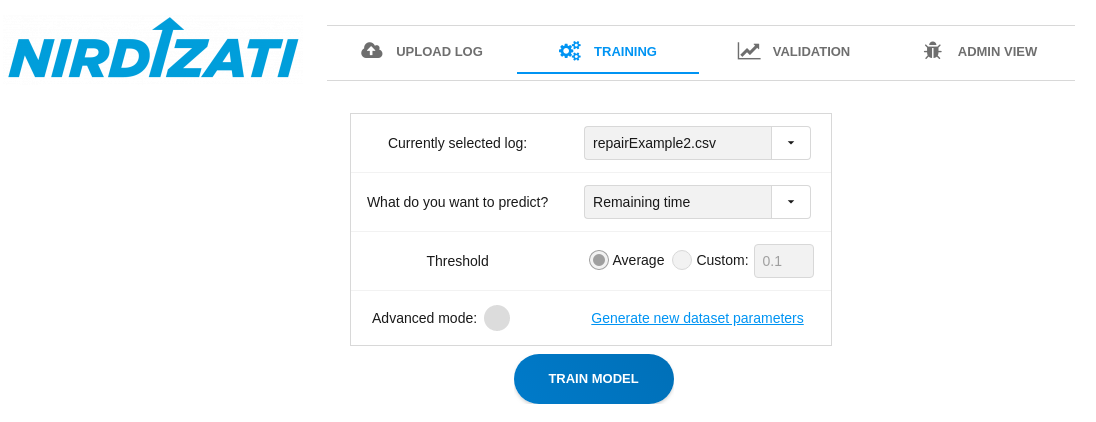
\includegraphics{figures/training.png}
        \end{tikzfigure}

        \begin{tikzfigure}[View of completed simulations, which allows sorting and grouping by various parameters.]
            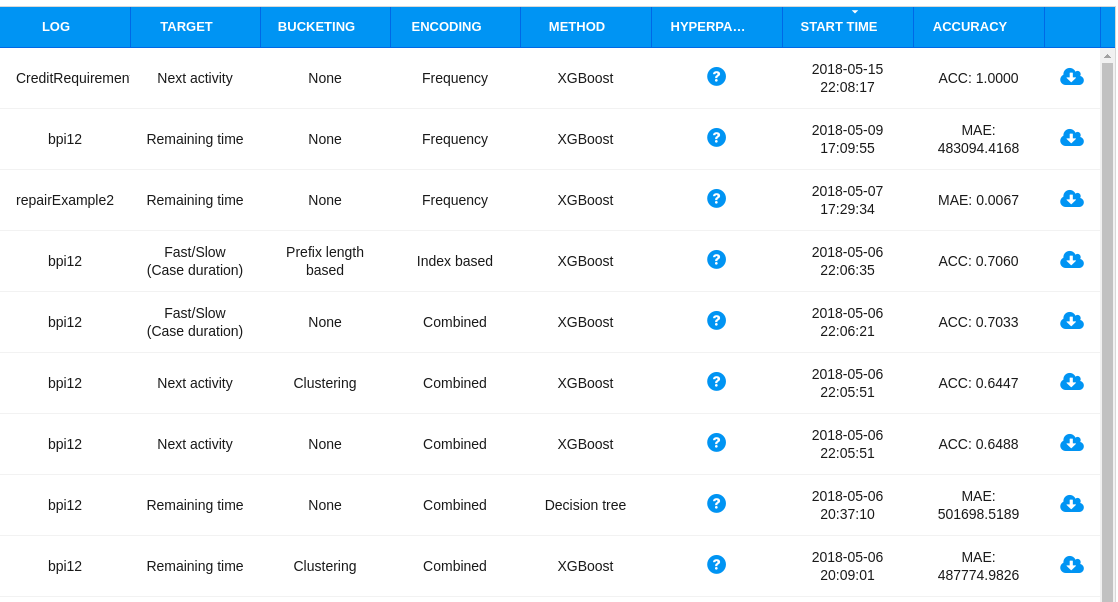
\includegraphics{figures/validation.png}
        \end{tikzfigure}

        \begin{tikzfigure}[Model evaluation view with model accuracy visualization.]
            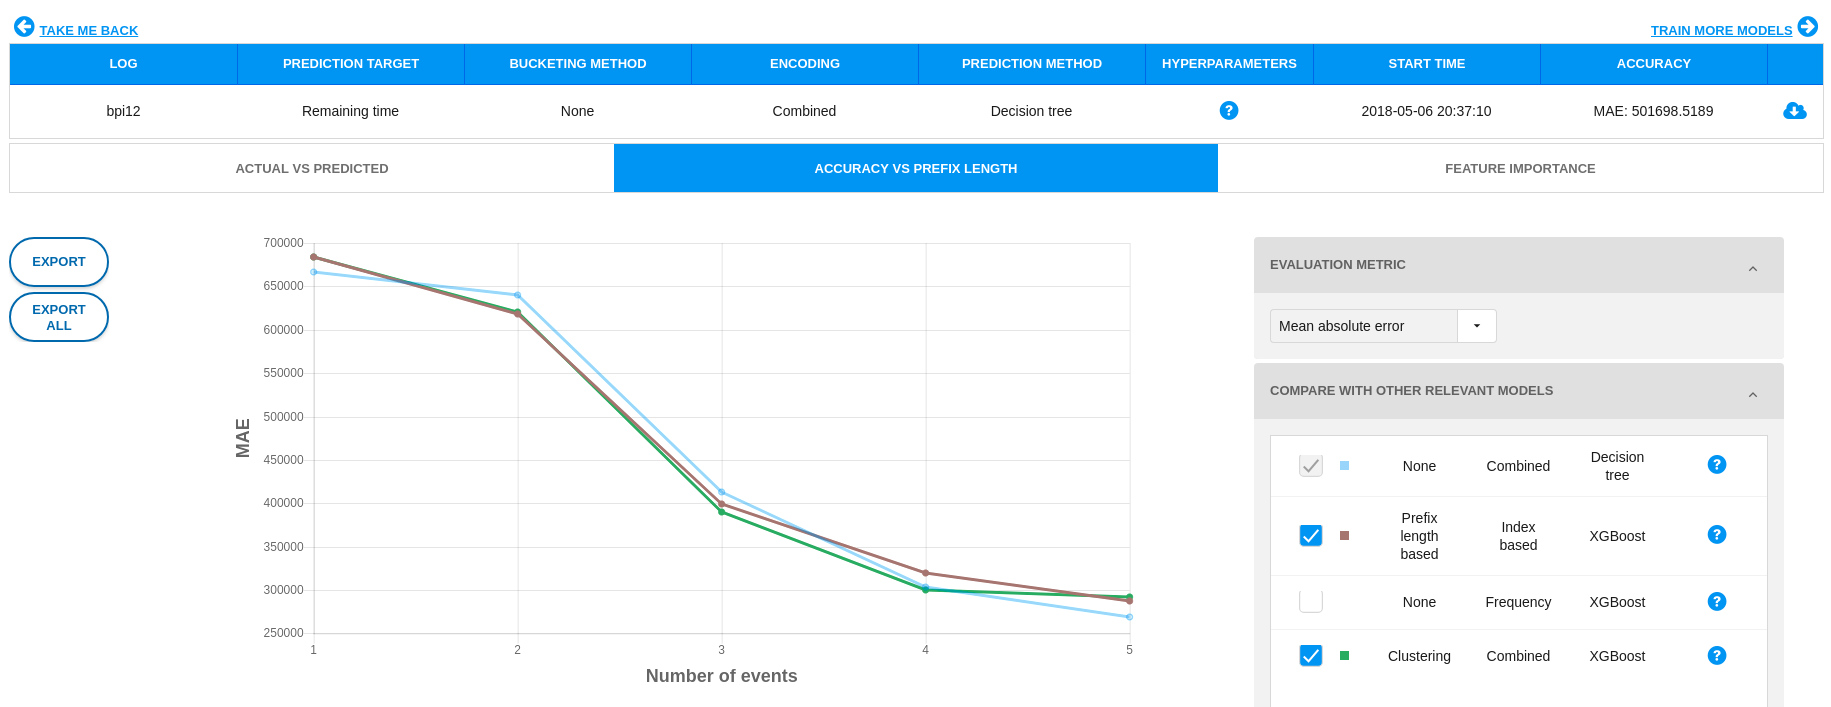
\includegraphics[scale=0.65]{figures/model_overview.png}
        \end{tikzfigure}
        }

        \column{0.3}
        \block{Technical solution}
        {
        Data flow diagram?
        Architecture diagram?
        }

        \block{Links}
        {
        \textbf{Code:} \href{https://github.com/Zukkari/nirdizati-training-ui}{\url{https://github.com/Zukkari/nirdizati-training-ui}}
        \bigbreak

        \textbf{Nirdizati:} \href{http://nirdizati.org/}{\url{http://nirdizati.org}}
        \bigbreak

        \textbf{Nirdizati Training:} \href{http://training.nirdizati.org/}{\url{http://training.nirdizati.org/}}
        \bigbreak

        \textbf{Twitter:} \href{https://twitter.com/nirdizati}{\url{https://twitter.com/nirdizati}}
        }
    \end{columns}
\end{document}